
%(BEGIN_QUESTION)
% Copyright 2009, Tony R. Kuphaldt, released under the Creative Commons Attribution License (v 1.0)
% This means you may do almost anything with this work of mine, so long as you give me proper credit

Read and outline the ``Calibration Errors and Testing'' section of the ``Instrument Calibration'' chapter in your {\it Lessons In Industrial Instrumentation} textbook.  Note the page numbers where important illustrations, photographs, equations, tables, and other relevant details are found.  Prepare to thoughtfully discuss with your instructor and classmates the concepts and examples explored in this reading.

\underbar{file i03908}
%(END_QUESTION)





%(BEGIN_ANSWER)


%(END_ANSWER)





%(BEGIN_NOTES)

A {\it zero shift} alters the $b$ term of an instrument's $y = mx + b$ function, resulting in the graph being shifted vertically from ideal.

\vskip 10pt

A {\it span shift} alters the $m$ term of an instrument's $y = mx + b$ function, resulting in the graph being at the wrong slope as compared to ideal.

\vskip 10pt

A {\it linearity} error causes the graphed function to not be a straight line.  Some instruments have linearity adjustements, while others do not.

\vskip 10pt

A {\it hysteresis} error causes the instrument to track differently with an increasing signal as opposed to a decreasing signal.  This is almost always caused by friction in some moving part of the instrument.  Instruments containing flexures may exhibit hysteretic behavior if the flexure becomes cracked or bent.

\vskip 10pt

Calibration errors usually come in more than one form at a time (e.g. zero and hysteresis, etc.).  Zero shift almost always accompanies a realistic calibration error, and so a simple one-point calibration check is often used as a quick method for detecting the presence of calibration errors: if the calibration checks out at one point, the zero is most likely good, which means the likelihood of other errors being present is low.  If an error is detected at any one point, recalibration is necessary.

\vskip 10pt

Differential pressure instruments equipped with 3-valve or 5-valve manifolds may be blocked and equalized to perform single-point checks.

\vskip 10pt

Instrument calibration is typically documented by the results of ``As-Found'' and ``As-Left'' tests (before and after any calibration adjustments).  These tests are usually conducted with the stimulus variable adjusted in both directions, in an ``up'' test as well as a ``down'' test.  Changing the direction of the variable's change is necessary to quantify hysteresis error.

\vskip 10pt

Some sophisticated instruments such as chemical analyzers have the ability to check their own calibrations, by switching solenoid valves on and off in such a way to subject the instrument to known quantities.  In the case of a gas analyzer, this takes the form of ``zero gas'' and ``span gas'' cylinders periodically routed to the input of the analyzer.  Semi-automated calibration may be enabled through the use of electronic documenting calibrator test equipment which automatically logs a technician's test results.  These devices interface with personal computers to archive the calibration data via calibration management software.  Certain industries such as those regulated by the US Food and Drug Administration must (by law) record all this data.













\vskip 20pt \vbox{\hrule \hbox{\strut \vrule{} {\bf Suggestions for Socratic discussion} \vrule} \hrule}

\begin{itemize}
\item{} What does it mean to ``split the error'' when encountering an instrument with a some nonlinearity?
\item{} Explain why an {\it up-down} test is essential when quantifying how much hysteresis an instrument has.
\item{} Suppose a mechanical gauge exhibits hysteresis when tested with a rising and a falling pressure stimulus.  How might you as a technician correct this calibration problem?
\item{} Provide an example of a {\it zero}, {\it span}, {\it linearity}, or {\it hysteresis} error, in the context of an automobile speedometer.
\item{} Provide an example of a {\it zero}, {\it span}, {\it linearity}, or {\it hysteresis} error, in the context of a baking thermometer.
\item{} Provide an example of a {\it zero}, {\it span}, {\it linearity}, or {\it hysteresis} error, in the context of a bathroom scale.
\item{} Explain why testing an instrument for a {\it zero} error is a good first step in determining whether {\it any} calibration errors exist.
\item{} Explain how to perform a single-point calibration check of a DP transmitter equipped with a 3-valve manifold.
\end{itemize}











\vfil \eject

\noindent
{\bf Prep Quiz:}

\vskip 10pt

Suppose an instrument technician uses a screwdriver to adjust the ``Z'' (zero) potentiometer on this analog pressure transmitter:

$$\includegraphics[width=15.5cm]{i03908x01.eps}$$

What effect will this calibration adjustment have on the equation describing the response of this transmitter?

$$y = mx + b$$

\begin{itemize}
\item{} This adjustment will change the value of $x$ 
\vskip 5pt 
\item{} This adjustment will change the value of $b$
\vskip 5pt 
\item{} This adjustment will change the value of $m$ 
\vskip 5pt 
\item{} This adjustment will change the sign of $m$ 
\vskip 5pt 
\item{} This adjustment will have no effect on the equation at all 
\end{itemize}


%INDEX% Reading assignment: Lessons In Industrial Instrumentation, Instrument Calibration

%(END_NOTES)


